\documentclass[xcolor=x11names,compress,aspectratio=169]{beamer}
%\documentclass[xcolor=x11names,compress,aspectratio=43]{beamer}

%% General document %%%%%%%%%%%%%%%%%%%%%%%%%%%%%%%%%%
\usepackage{graphicx}
\usepackage{tikz}
\usepackage{amsmath}
\usepackage{amssymb}
\usepackage[utf8]{inputenc}
\usepackage{textpos}
\usepackage{booktabs}
\usepackage{listings}
\usepackage{auto-pst-pdf}

\usetikzlibrary{decorations.fractals, calc}
%%%%%%%%%%%%%%%%%%%%%%%%%%%%%%%%%%%%%%%%%%%%%%%%%%%%%%

%% Beamer Layout %%%%%%%%%%%%%%%%%%%%%%%%%%%%%%%%%%
\useoutertheme[subsection=false,shadow]{miniframes}
\useinnertheme{default}
%\usefonttheme{serif}
\usepackage{palatino}
\setbeamerfont{title like}{shape=\scshape}
\setbeamerfont{frametitle}{shape=\scshape}
\beamertemplatenavigationsymbolsempty


% Uncomment this line, if you want frame numbers on your slides
% (I disabled them since I had the progress bar at the header)
%\setbeamertemplate{footline}[frame number]

\definecolor{fmiBlue}{RGB}{11,128,145} % FSU Faculty blue
\definecolor{evbc}{RGB}{50,167,132} % EVBC Green
\definecolor{bgGray}{RGB}{230,230,230} % some gray if needed


\setbeamercolor*{upper separation line head}{bg=Snow4} %Snow4 comes from the x11names option of xcolor
%\setbeamercolor*{lower separation line head}{bg=evbc}  % obsolete - there is now a cool progress bar 
\setbeamercolor*{normal text}{fg=black,bg=white} 
\setbeamercolor*{alerted text}{fg=red} 
\setbeamercolor*{example text}{fg=black} 
\setbeamercolor*{structure}{fg=black} 
 
\setbeamercolor*{palette tertiary}{fg=black,bg=black!10} 
\setbeamercolor*{palette quaternary}{fg=black,bg=black!10} 

%%%%%%%%%%%%%%%%%%%%%%%%%%%%%%%%%%%%%%%%%%%%
% IMPORTANT
% Kevin:
% Currently the FMI blue (the light uni blue) is here.
% If you want for example the evbc green, you'd have to
% change the colors here. I will put this in a nice function
% at some point.
\setbeamercolor{title}{fg=evbc}
\setbeamercolor{structure}{fg=evbc}
\setbeamercolor{frametitle}{fg=evbc}
\setbeamercolor{block title}{fg=evbc, bg=bgGray}
\setbeamercolor{block title example}{fg=evbc}
\setbeamercolor{enumerate item}{fg=evbc}
\setbeamercolor{itemize item}{fg=evbc}
\setbeamercolor{item projected}{bg=evbc}

\setbeamerfont{block title}{size=\small}
\setbeamerfont{block body}{size=\scriptsize}

% Use those if you want. Just some shortcuts for 
% columns. Personally, I use minipages nowadays.
\renewcommand{\(}{\begin{columns}}
\renewcommand{\)}{\end{columns}}
\newcommand{\<}[1]{\begin{column}{#1}}
\renewcommand{\>}{\end{column}}

% Kevin:
% This is used for the code examples in the document.
% If used, set the frame option to 'fragile' (!!!)
\lstset{
	language=sh, 
	numbers=left, 
	numberstyle=\tiny\color{gray}, 
	backgroundcolor=\color{bgGray}, 
	basicstyle=\scriptsize\ttfamily,
	commentstyle=\tiny\color{Green4},
	keywordstyle=\color{Blue3},
	escapeinside=@@
}

% Kevin
% Appendix page number fix. More like an ugly hack.
% I was never able to create a "nice" appendix command, however, this one here works fine.
\newcommand{\beginbackup}{
   \newcounter{framenumbervorappendix}
   \setcounter{framenumbervorappendix}{\value{framenumber}}
}
\newcommand{\backupend}{
   \addtocounter{framenumbervorappendix}{-\value{framenumber}}
   \addtocounter{framenumber}{\value{framenumbervorappendix}} 
}

%%%%%%%%%%%%%%%%%%%%%%%%%%%%%%%%%%%%%%%%%%%%%%%%%%
% Kevin: Change this, if you want.
\graphicspath{{figures/}}
%

% Kevin:
% I used this slides for subsections a long time ago, however, at some point I figured that it is nicer to have those slides
% at the beginning of each section. Use this extra slides to give a short summary of the previous talk.
\AtBeginSection[]{
  \begin{frame}
  \vfill
  \centering
  \begin{beamercolorbox}[sep=8pt,center,shadow=true,rounded=true]{title}
    \usebeamerfont{title}\insertsection\par%
  \end{beamercolorbox}
  \vfill
  \end{frame}
}


% Kevin:
% small macro, used to build the progress bar
\def\insertframeratio{%
    \pgfmathparse{\insertframenumber/\inserttotalframenumber}%
}
%%%%%%%%%%%%%%%%%%%%%%%%%%
% Kevin:
% This is the progress bar in the headline.
% Change the textcolor if needed, change the width to 2pt if wanted
\addtobeamertemplate{headline}{}{%
  \insertframeratio
  \edef\myvar{\pgfmathresult}
  %\textcolor{evbc}{\rule{\myvar \paperwidth}{1pt}}
  \textcolor{evbc}{\rule{\paperwidth}{1pt}}
}

%%%%%%%%%%%%%%%%%%%%%%%%%%%
% Kevin
% This adds the FSU Logo to the
% bottom left. Changing the logo is easy
% adding a second logo (e.g. the evbc) is tricky
\addtobeamertemplate{footline}{}{%
\begin{textblock*}{100mm}(1em,-3.5em)

\includegraphics[scale=0.4]{evbc_cmyk.pdf}
\end{textblock*} 
\begin{textblock*}{100mm}(73em,-1em) 
\insertframenumber/\inserttotalframenumber
\end{textblock*}
}

%% Kevin:
%% I used this in order to show two logos at the same time.
%% as you can see, it is quite tricky in terms of positioning 
%% and size, but a nice try-and-error session usually
%% works out.
%\addtobeamertemplate{footline}{}{%
%\begin{textblock*}{100mm}(0.5em,-5em)
%
\includegraphics[scale=0.5]{figures/evbc_cmyk.pdf}
%\end{textblock*}
%\begin{textblock*}{100mm}(11em,-3em)
%
\includegraphics[scale=0.025]{fsu_logo.jpg}
%\end{textblock*}
%}


% Kevin:
% Well, fill this out as needed
%\title{Theoretical and practical metagenomic approaches to viral discovery}
%\subtitle{}
%\author{Kevin Lamkiewicz, Manja Marz}
%\date{27.09.2018\\[1em]RNA Bioinformatics and High-Throughput Analysis\\[1em]Friedrich Schiller University Jena}
%\date{xx.xx.2018\\RNA Bioinformatics and High-Throughput Analysis\\[2em]
\includegraphics[scale=0.05]{fsu_logo.jpg}}



\title{Theoretical and practical metagenomic approaches to viral discovery}
\subtitle{Practical Session: ViennaRNA on single molecules}
\author{Kevin Lamkiewicz, Manja Marz}
\date{24.10.2019\\[1em]European Virus Bioinformatics Center}

\begin{document}

\begin{frame}
  \maketitle
\end{frame}

\section[Intro]{Introducing ViennaRNA}

\begin{frame}[c]\frametitle{Nothing in common!}
  \begin{center}
      
\includegraphics[width=1\textwidth]{figures/sequence_sim.pdf}
  \end{center}
\end{frame}

\begin{frame}[c]\frametitle{Tools and Scripts}
    
  \begin{itemize}
      \item<2-> \texttt{ViennaRNA}
      \uncover<2->{
      \begin{itemize}
          \item \texttt{RNAfold}
          \item \texttt{RNAsubopt}
          \item \texttt{RNAcofold}
          \item \texttt{RNAduplex}
          \item \texttt{RNAalifold}
          \item \texttt{RNALfold}
          \item \texttt{$\dots$}
      \end{itemize}
      }

      \item<3-> \texttt{LocaRNA}
      \item<4-> \texttt{MAFFT}, \texttt{VARNA}, $\dots$
  \end{itemize}
\end{frame}

\section[RNAfold]{Hands on!}

\begin{frame}[c, fragile]\frametitle{RNAfold}
  \begin{overlayarea}{\textwidth}{0.5\textheight}
  \begin{lstlisting}
# Use RNAfold on sequence.fasta in order 
# to fold all sequences in the file
$> RNAfold  < sequence.fasta
  \end{lstlisting}    

  \begin{onlyenv}<2->%
  \begin{lstlisting}
# Redirect the output of RNAfold into a file
$> RNAfold  < sequence.fasta > sequence.fold
  \end{lstlisting}            
  \end{onlyenv}
  \end{overlayarea}
\end{frame}

\begin{frame}[c, fragile]\frametitle{RNAfold mit Partition Function}
  \begin{lstlisting}
# Use the -p parameter to calculate the partition function
# on top of the minimum free energy secondary structures
$> RNAfold -p < sequence.fasta > sequence.fold  
@\pause@
# This will produce a centroid structure; 
# the structure with minimal average distance to all 
# sampled structures.
# . unpaired
# , weakly paired
# | strongly paired w/o preference
# { } weakly paired
# ( ) strongly paired
  \end{lstlisting}
\end{frame}

\begin{frame}[t, fragile]\frametitle{MEA structure}
  \begin{block}{Maximum expected accuracy Structure}
      Reminder: With the \emph{partition function} we are able to calculate basepair probabilities.
      The structure with the heighest sum of all probabilities, is called the \emph{MEA structure}.
  \end{block}

  \begin{onlyenv}<2>
   \hfill
  \begin{lstlisting}
# Use -p and --MEA to calculate the MFE,
# the MEA and the centroid structure.
# Note: The MFE and the MEA structure do not have to be the same!
# Note2: --MEA usually implies -p
$> RNAfold -p --MEA < sequence.fasta > sequence.fold
  \end{lstlisting}
\end{onlyenv}
\end{frame}

\begin{frame}[c,fragile]\frametitle{Structure and Dotplots}
  
  \begin{lstlisting}
# the same command again; you will get an rna.ps and a dot.ps
$> RNAfold -p --MEA < sequence.fasta > sequence.fold
  \end{lstlisting}
  

  \begin{minipage}{0.4\textwidth}
      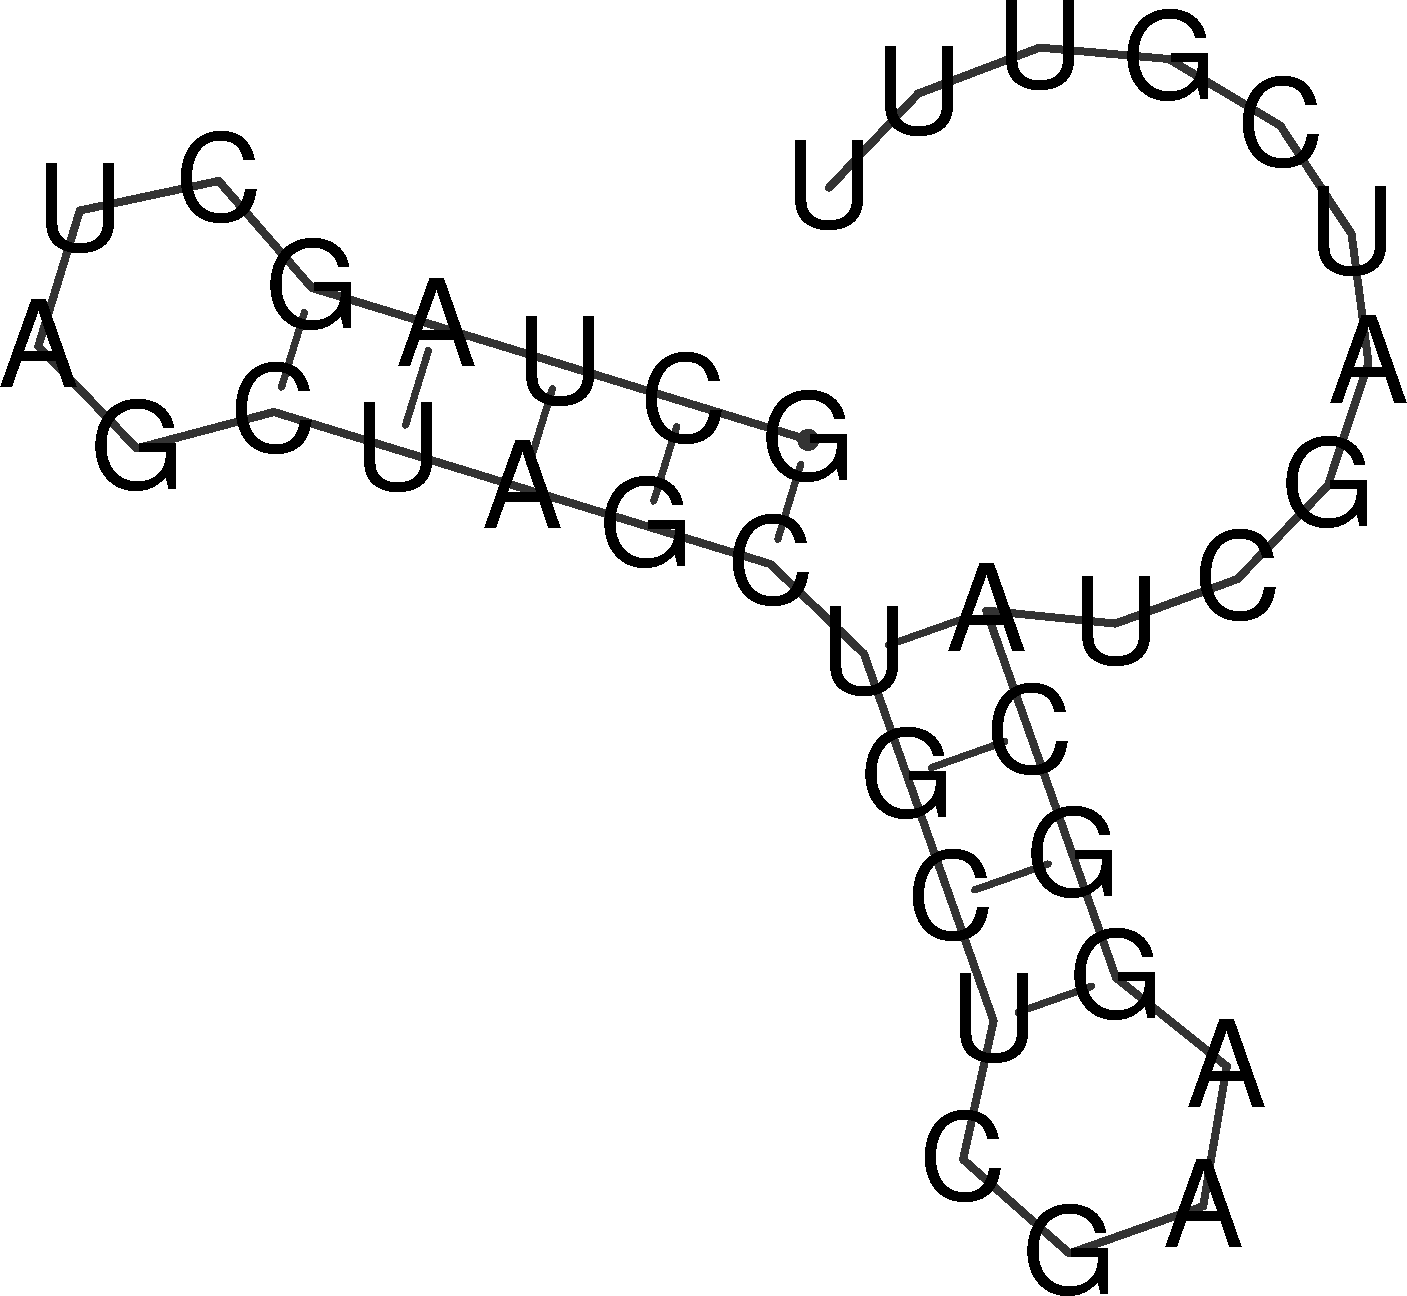
\includegraphics[width=0.8\textwidth]{figures/rna.pdf}
  \end{minipage} \hfill \begin{minipage}{0.4\textwidth}
      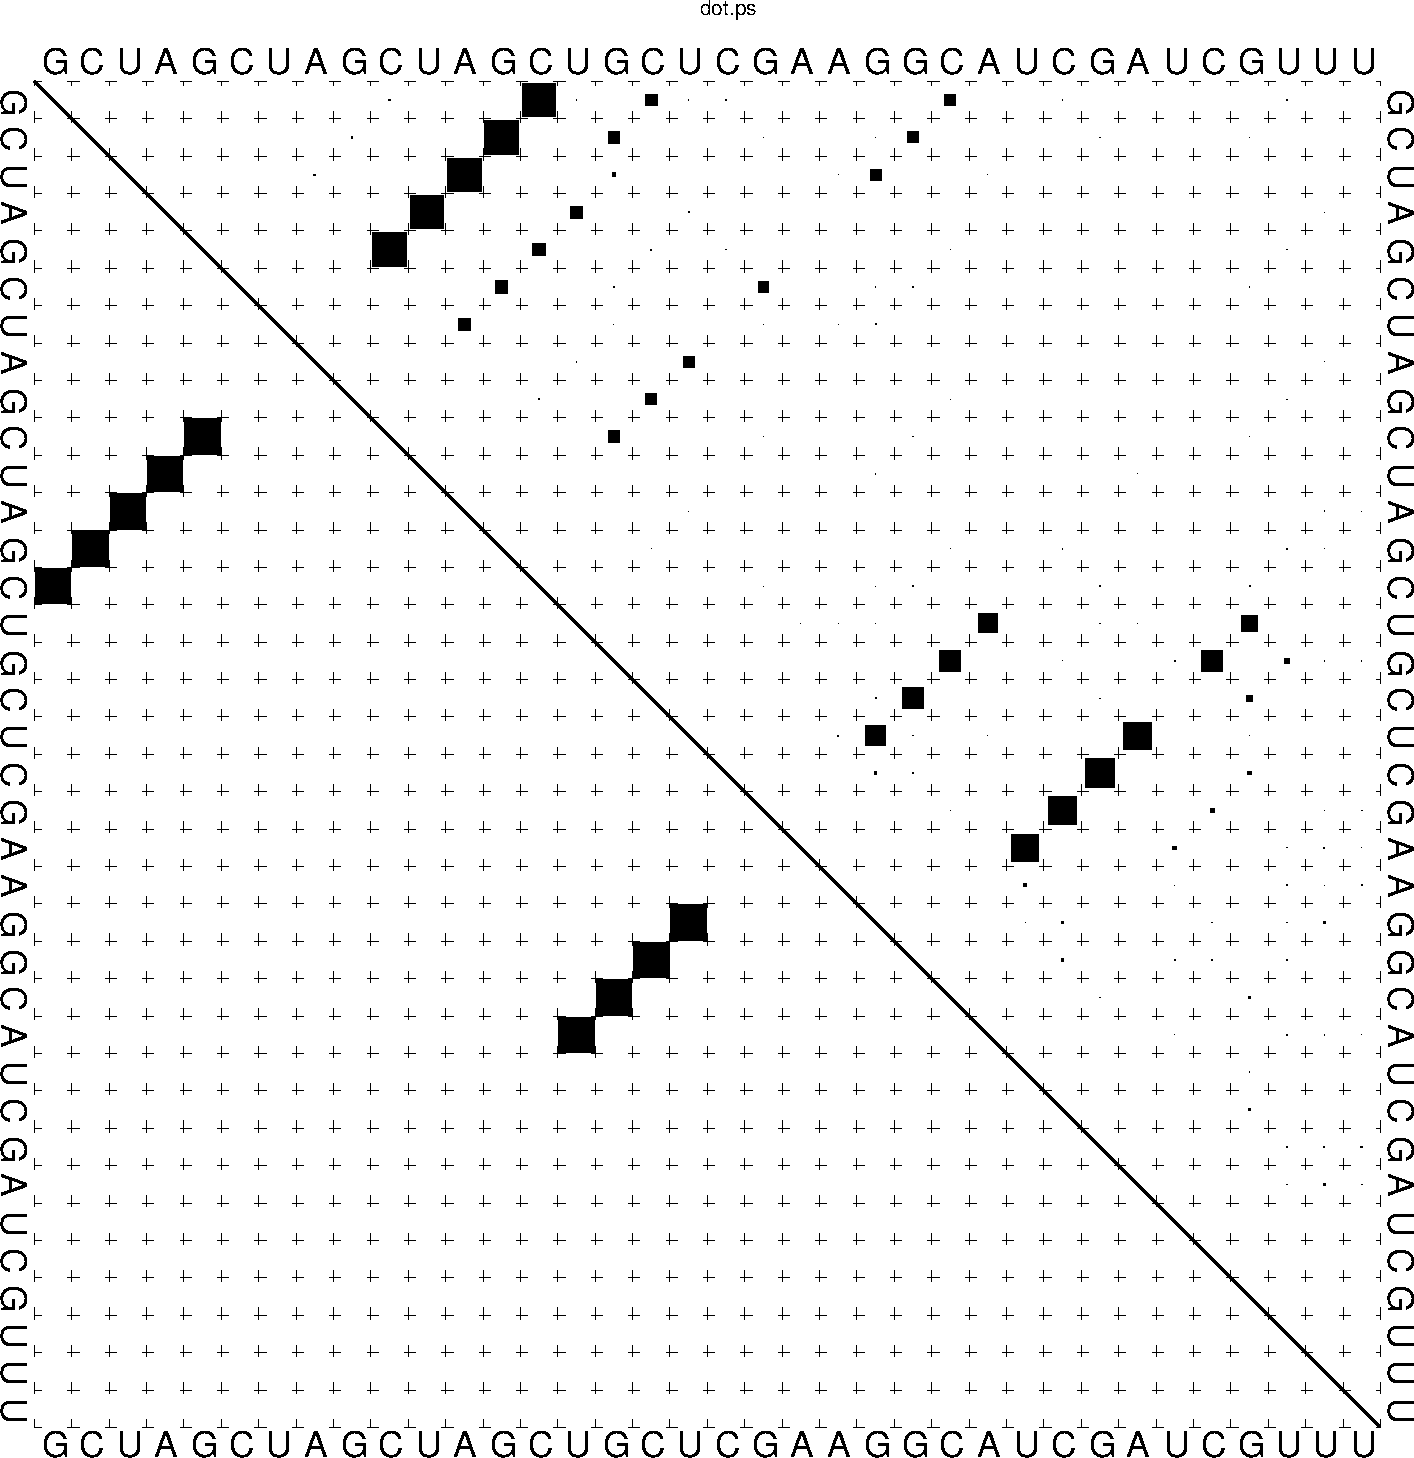
\includegraphics[width=0.8\textwidth]{figures/dot.pdf}
  \end{minipage}
\end{frame}


\begin{frame}[t, fragile]\frametitle{RNAfold+}
  
  \begin{block}{Let's use some colors!}
      The \texttt{ViennaRNA Package} offers some \texttt{Perl}-scripts, which can enrich the PostScript files of our structures.
  \end{block}
  \vfill
  
  \uncover<2->{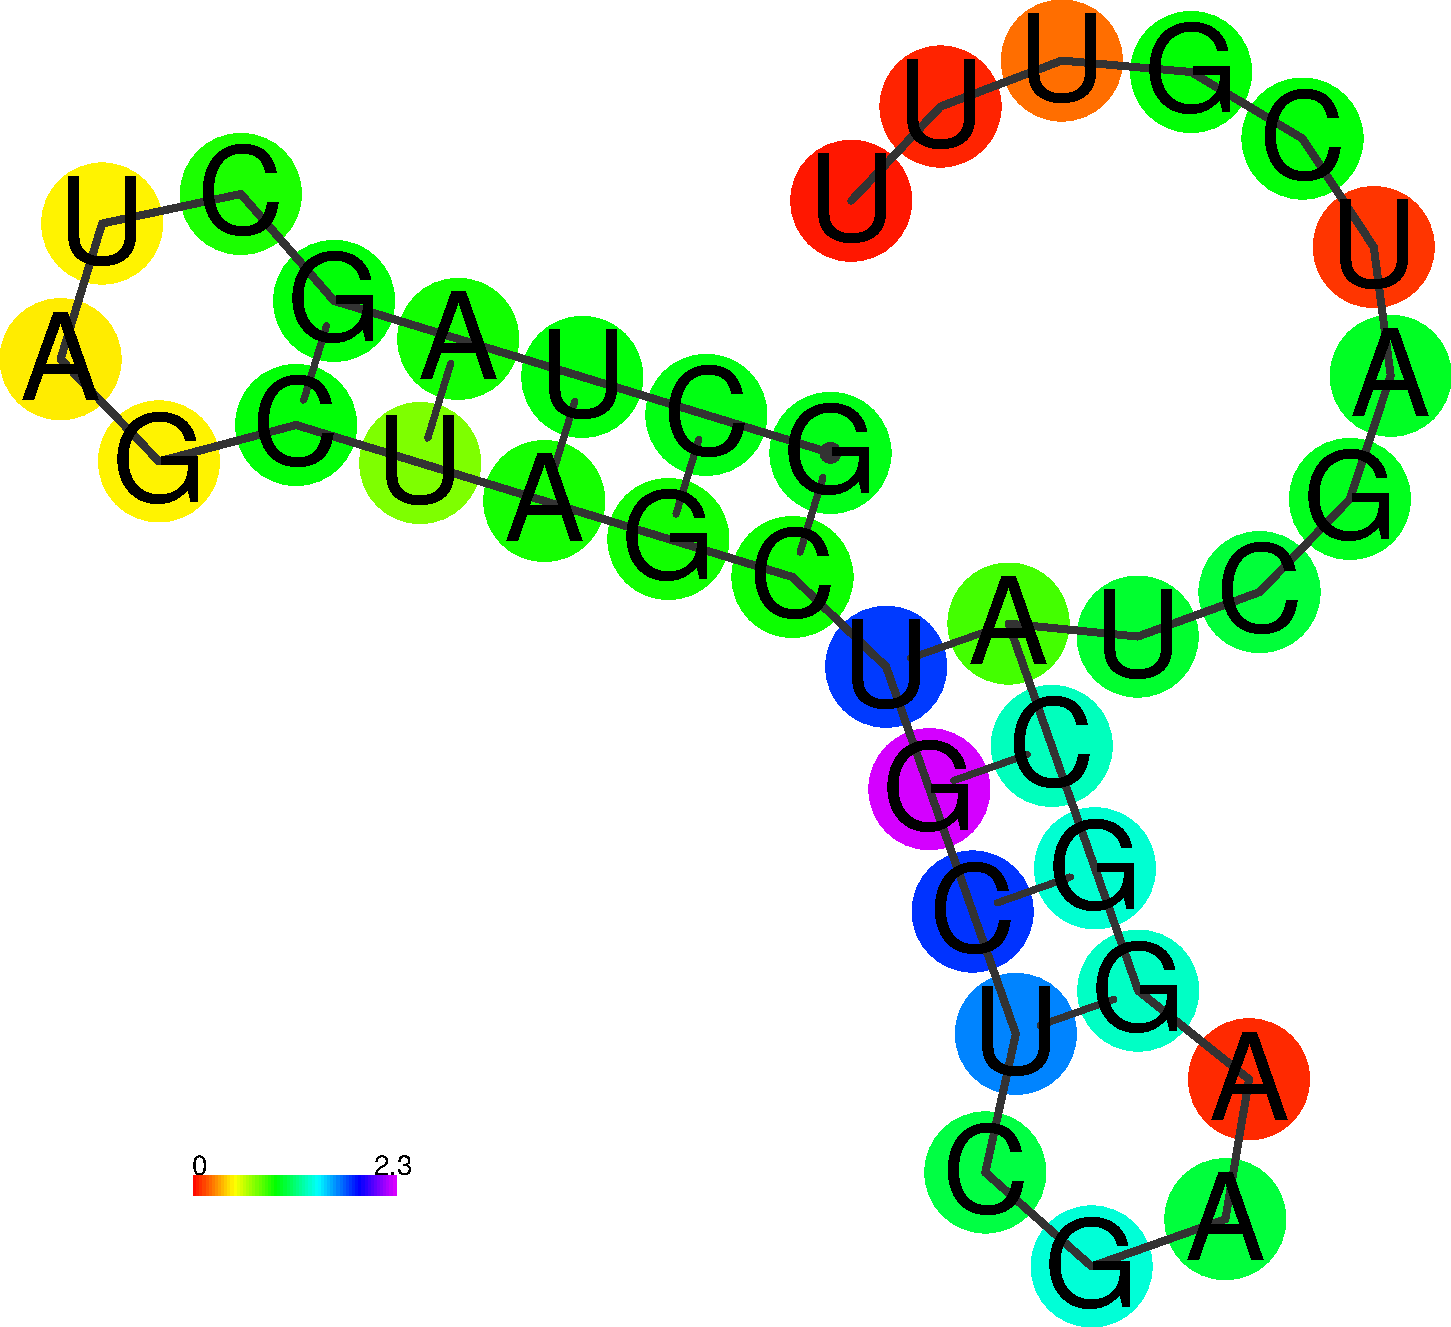
\includegraphics[width=0.3\textwidth]{figures/entropy.pdf}} \hfill
  \uncover<3->{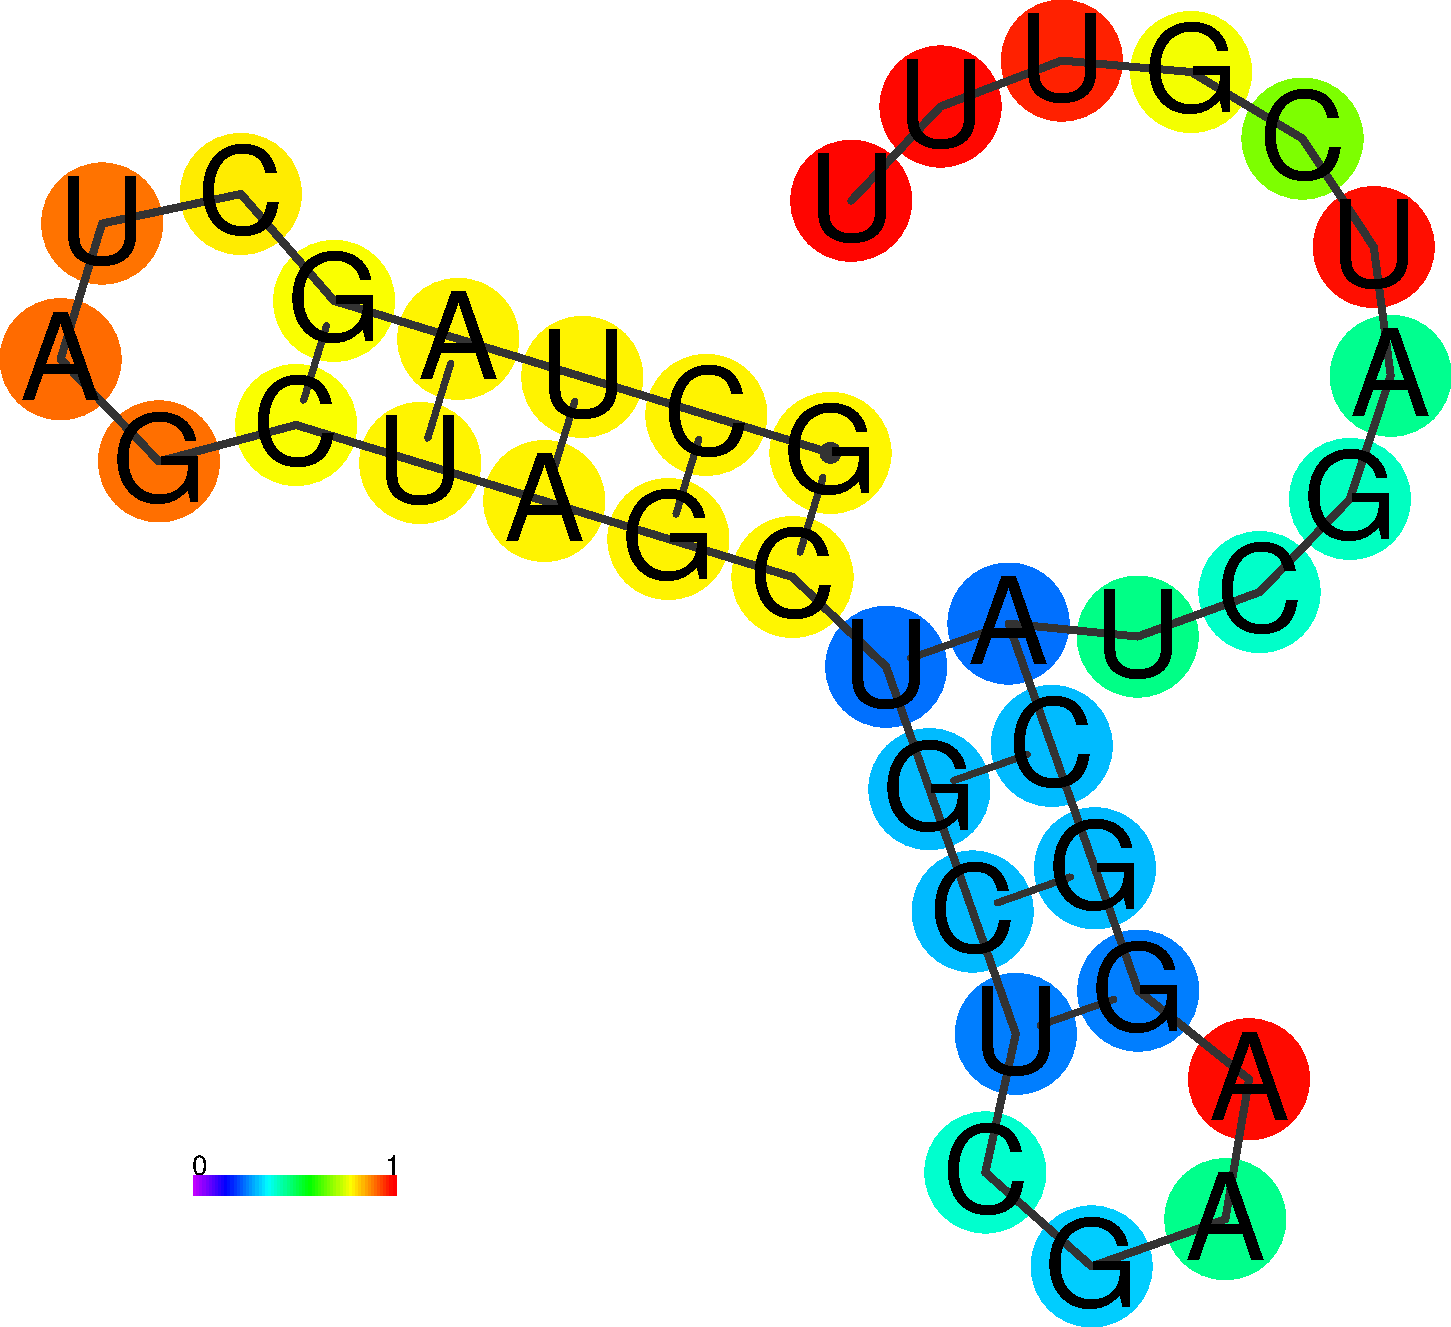
\includegraphics[width=0.3\textwidth]{figures/probability.pdf}} \hfill
  \uncover<4>{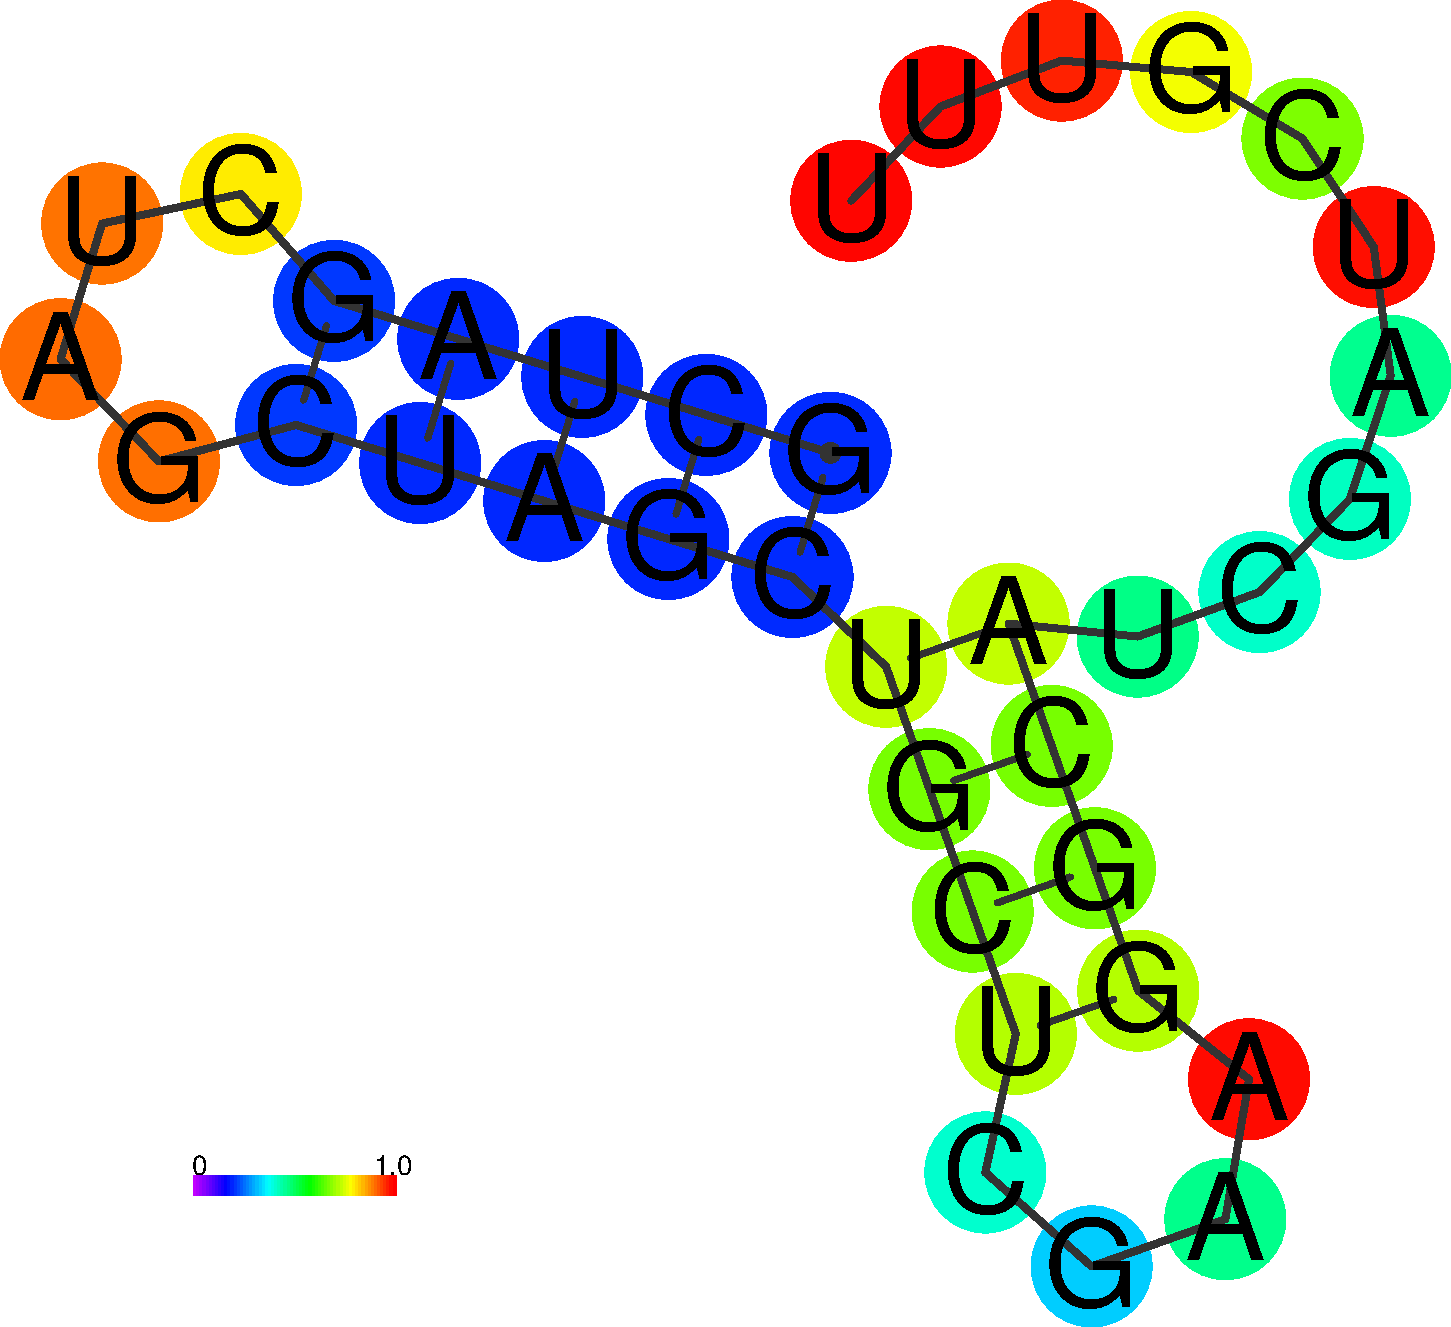
\includegraphics[width=0.3\textwidth]{figures/access.pdf}}
  
  
\end{frame}

\begin{frame}[c, fragile]\frametitle{RNAfold Perl Scripts}
  \begin{lstlisting}
# Low entropy regions have little structural flexibility, 
# which means the reliability of the predicted structure is high.
# High entropy indicate many structual alternatives
# which might be functional important but make the prediction
# more difficult - and thus less reliable.
$> ./relplot.pl rna.ps dot.ps > entropy.ps
@\pause@
# -p colors the nucleotides based on their base-pairing
# probability
$> ./relplot.pl -p rna.ps dot.ps > probability.ps
@\pause@
# -a colors the nucleotides based on their accessbility
# (e.g. the probability of being unpaired)
$> ./relplot.pl -a rna.ps dot.ps > access.ps
  \end{lstlisting}
\end{frame}

\section[Plausible Structures]{Suboptimal Structures and Constraints}

\begin{frame}[c, fragile]\frametitle{RNAsubopt}
\begin{overlayarea}{\textwidth}{0.7\textheight}
Sometimes we're interested in suboptimal structures.

  \begin{lstlisting}
# In general RNAsubopt is used exactly like RNAfold.
# With -p one calculates the partition function
$> RNAsubopt [OPTIONS] < sequence.fasta > sequence.subopt
@\pause@
# With the -e parameter, one can define a certain
# energy range. Using this, RNAsubopt returns
# all structures that are in range of this parameter.
$> RNAsubopt -e 2 < sequence.fasta > sequence_e2.subopt
  \end{lstlisting}
\end{overlayarea}

\end{frame}

\begin{frame}[c, fragile]\frametitle{RNAfold with constraints}
  \begin{itemize}
      \item Structure of RNA is partly known (e.g. via SHAPE experiments)
      \item \texttt{RNAfold} is able to consider this knowledge
  \end{itemize}

  \begin{lstlisting}
# Enable -C to include constraints. --noPS prevents the generation
# of the rna.ps and dot.ps files.
$> RNAfold --noPS -C < constrained.fasta > constrained.fold
@\pause@
# . (no constraint for this base)
# | (corresponding base has to be paired)
# x (base is unpaired)
# < (base i is paired with base j>i)
# > (base i is paired with base j<i)
# and matching brackets ()  (base i pairs with base j)
  \end{lstlisting}
\end{frame}


\section[Alignments]{Calculating structures alignment-based}

\begin{frame}[c, fragile]\frametitle{RNAalifold}
  \texttt{RNAalifold} calculates a \emph{consensus} RNA secondary structure for several aligned RNA sequences.
\begin{lstlisting}
# RNAalifold accepts CLUSTAL, Stockholm, FASTA or MAF
# formats for the input alignment.
# --color will produce a colored version of the structure plot
# --aln produces a colored alignment based on the structure

$> RNAalifold --aln --color < input.aln > consensus.alifold
\end{lstlisting}
\end{frame}

\begin{frame}[c, fragile]\frametitle{LocARNA vs MAFFT}
  In order to create a multiple sequence alignment, we can use \texttt{MAFFT} and/or \texttt{LocARNA} (and many more...)
  \begin{lstlisting}
# mafft creates a multiple sequence alignment based on
# sequence conservation only
$> mafft --clustalout cov_5utr.fa > cov_5utr_mafft.aln

# locarna folds and aligns the sequences simultanously,
# yielding better results for sequence that share a
# structural conservation
# However, locarna needs quite some time compared to sequence-based 
# alignment tools.
$> mlocarna --thread 4 cov_5utr.fasta > cov_5utr.locarna
  \end{lstlisting}   
\end{frame}

\begin{frame}[c, fragile]\frametitle{RNAalifold Results}
  \begin{lstlisting}
# alirna.ps and aln.ps give information of the structural conservation
$> RNAalifold --aln --color < cov_5utr_mafft.aln \ 
      > cov_5utr_mafft.alifold

# NOTE: both PostScript files will be overwritten!
# locarna saves the alignment in a subdirectory
$> RNAalifold --aln --color < cov_5utr.out/results/result.aln \ 
      > cov_5utr_locarna.alifold
  \end{lstlisting}
\end{frame}

\begin{frame}[c]\frametitle{Structures}
      
      \centering
      \only<1>{\texttt{MAFFT}\\
      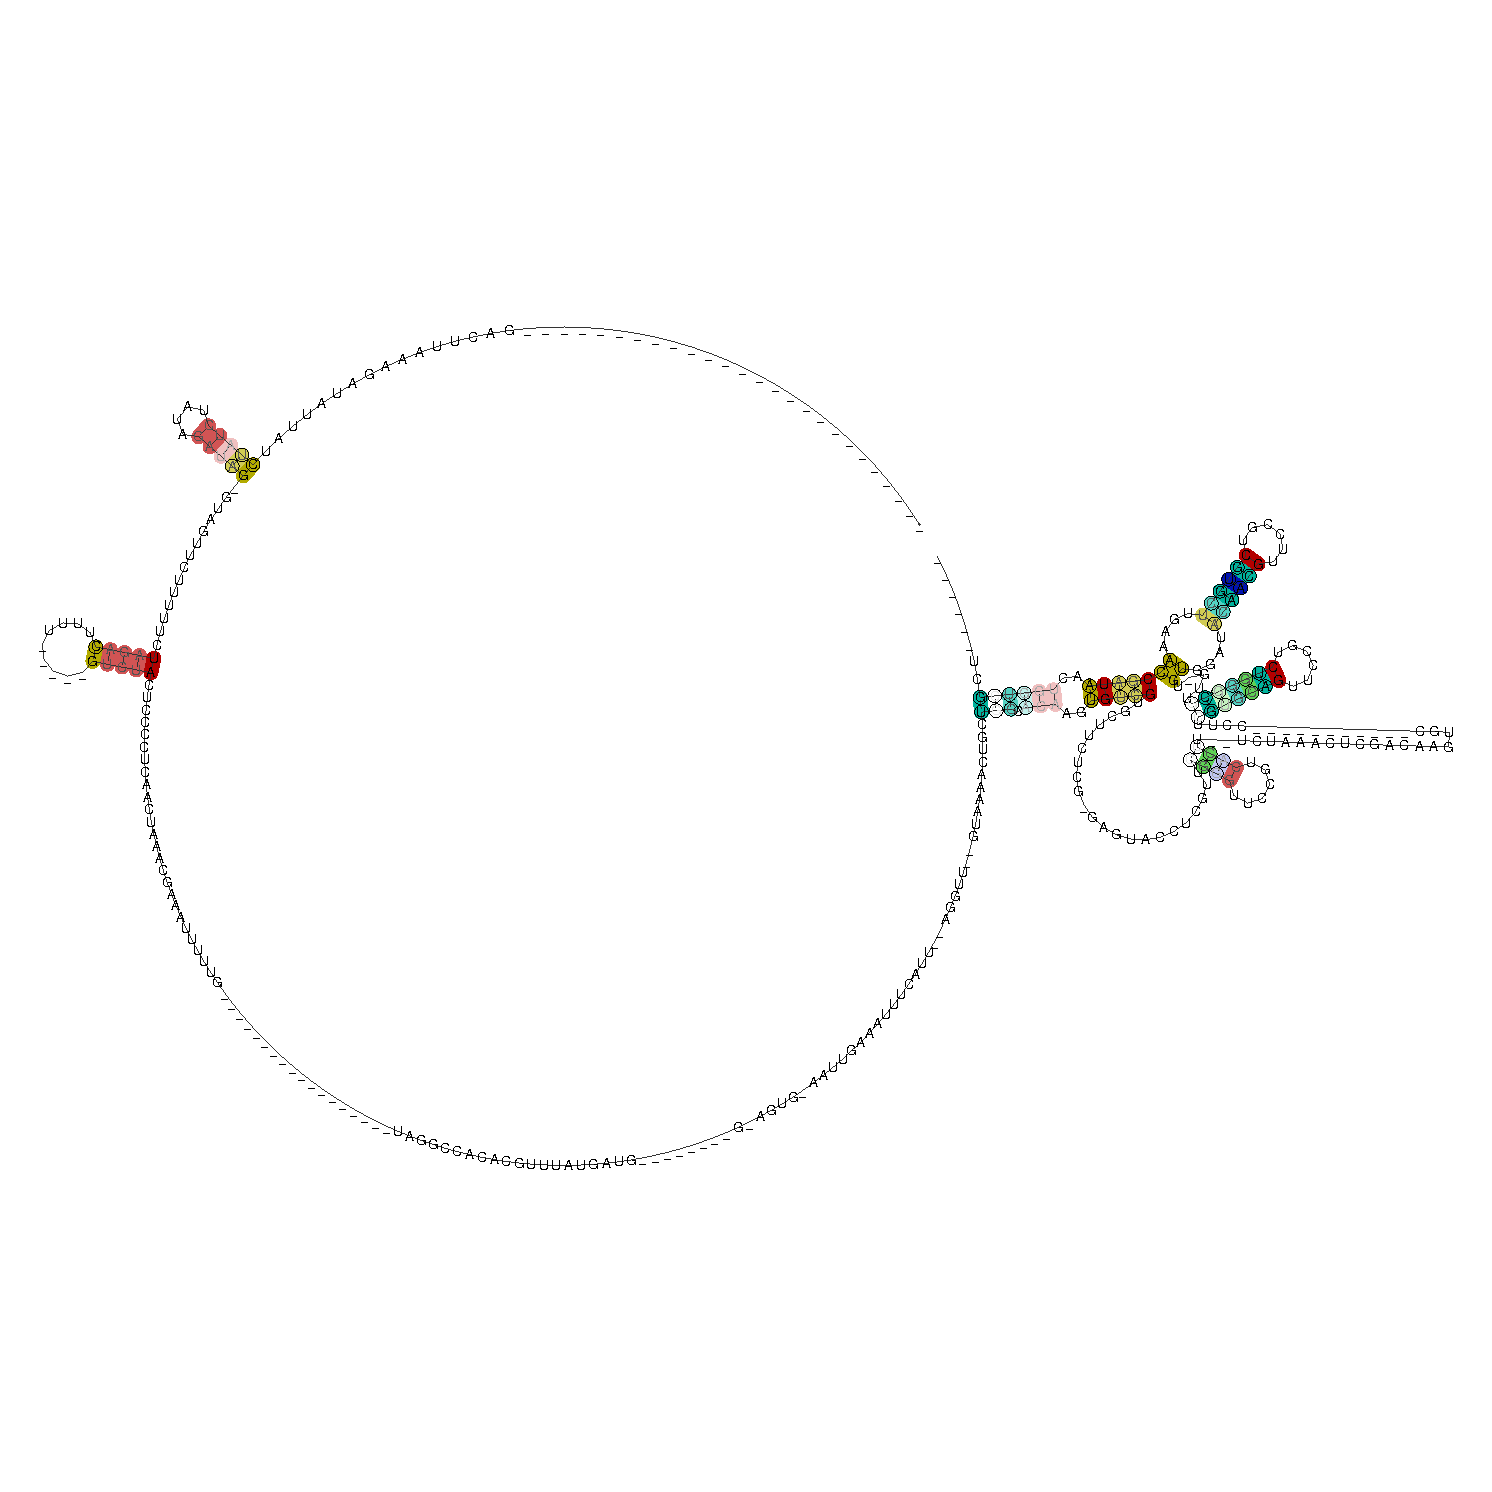
\includegraphics[width=0.6\textwidth]{figures/alirna_mafft.ps}}
      \only<2>{\texttt{LocARNA}\\
      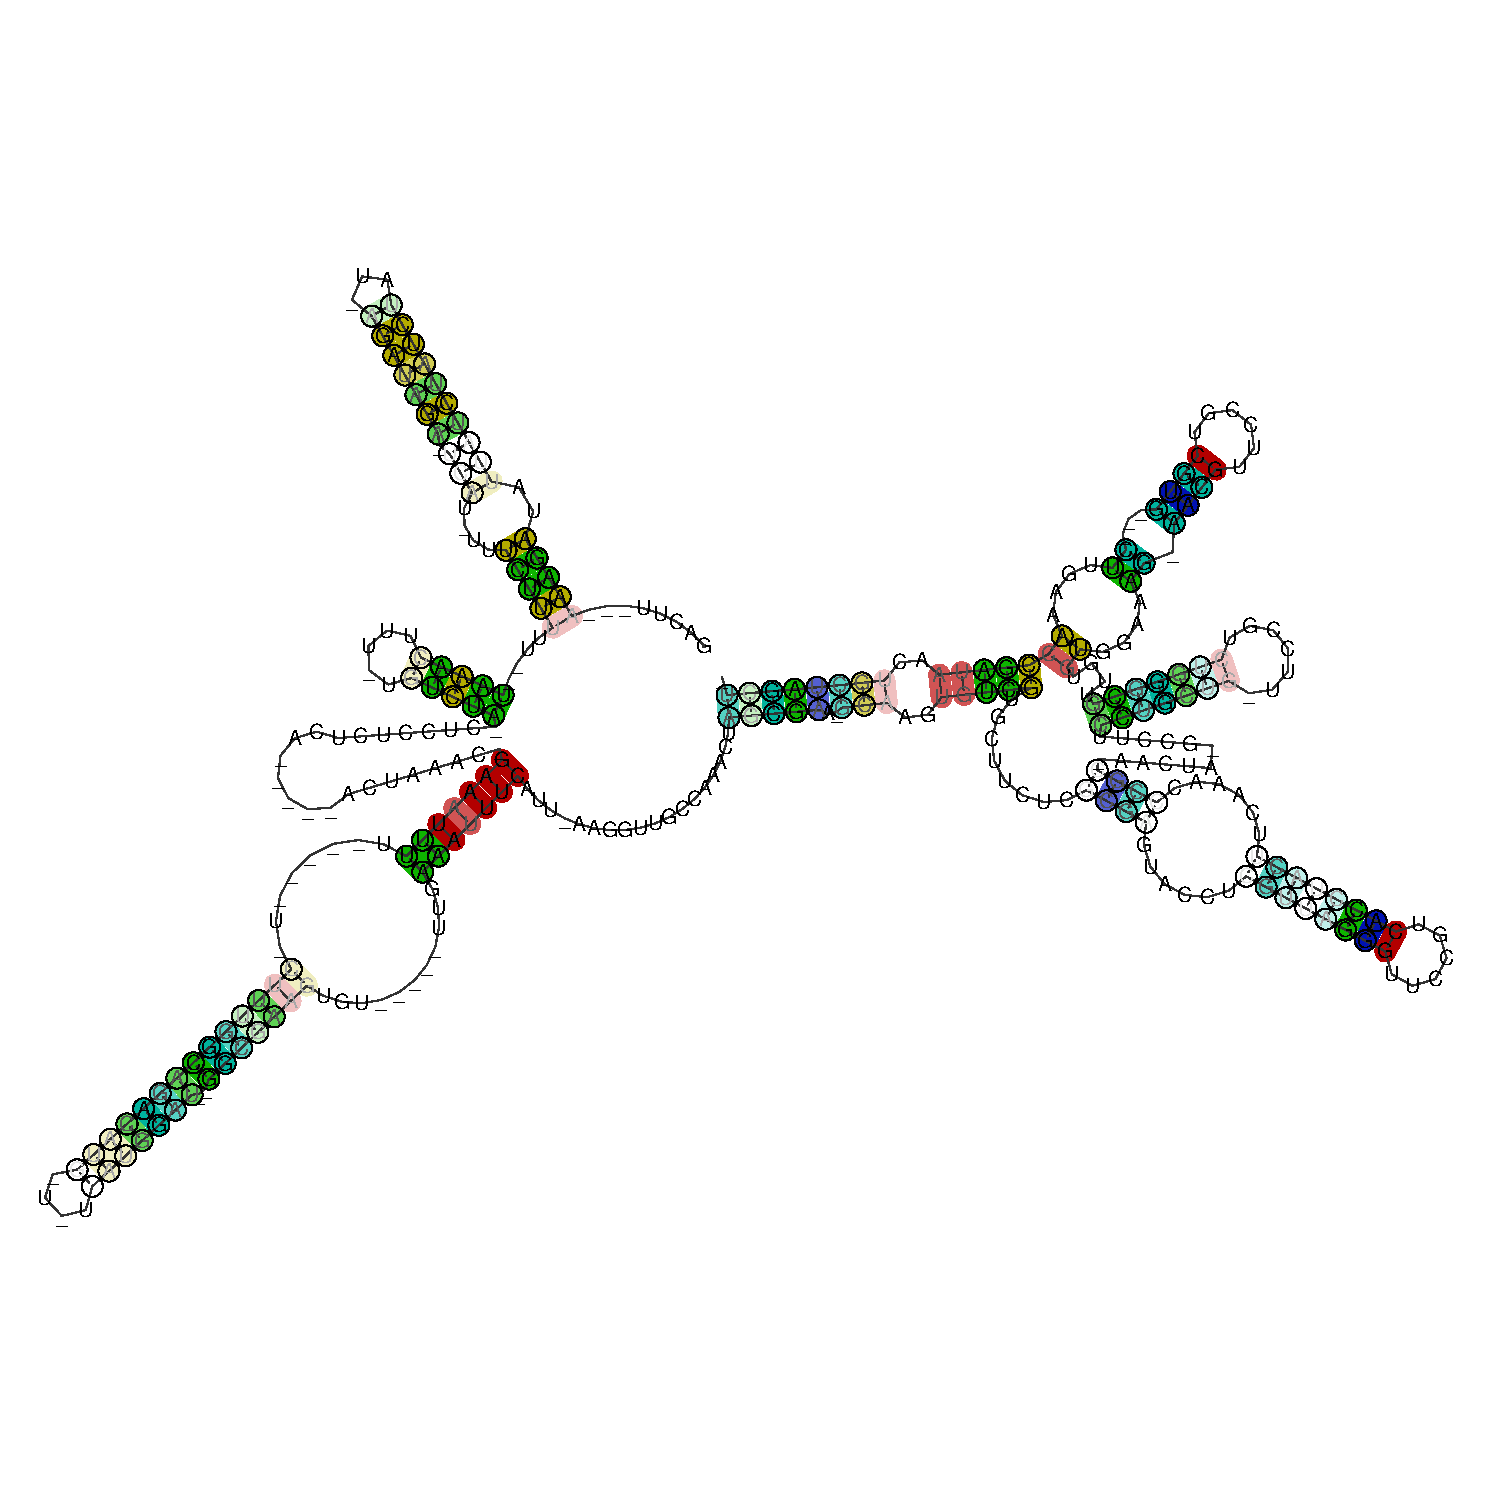
\includegraphics[width=0.6\textwidth]{figures/alirna_locarna.ps}}

      \only<3->{
      \begin{minipage}{0.45\textwidth}
      \centering
      \texttt{MAFFT}\\
      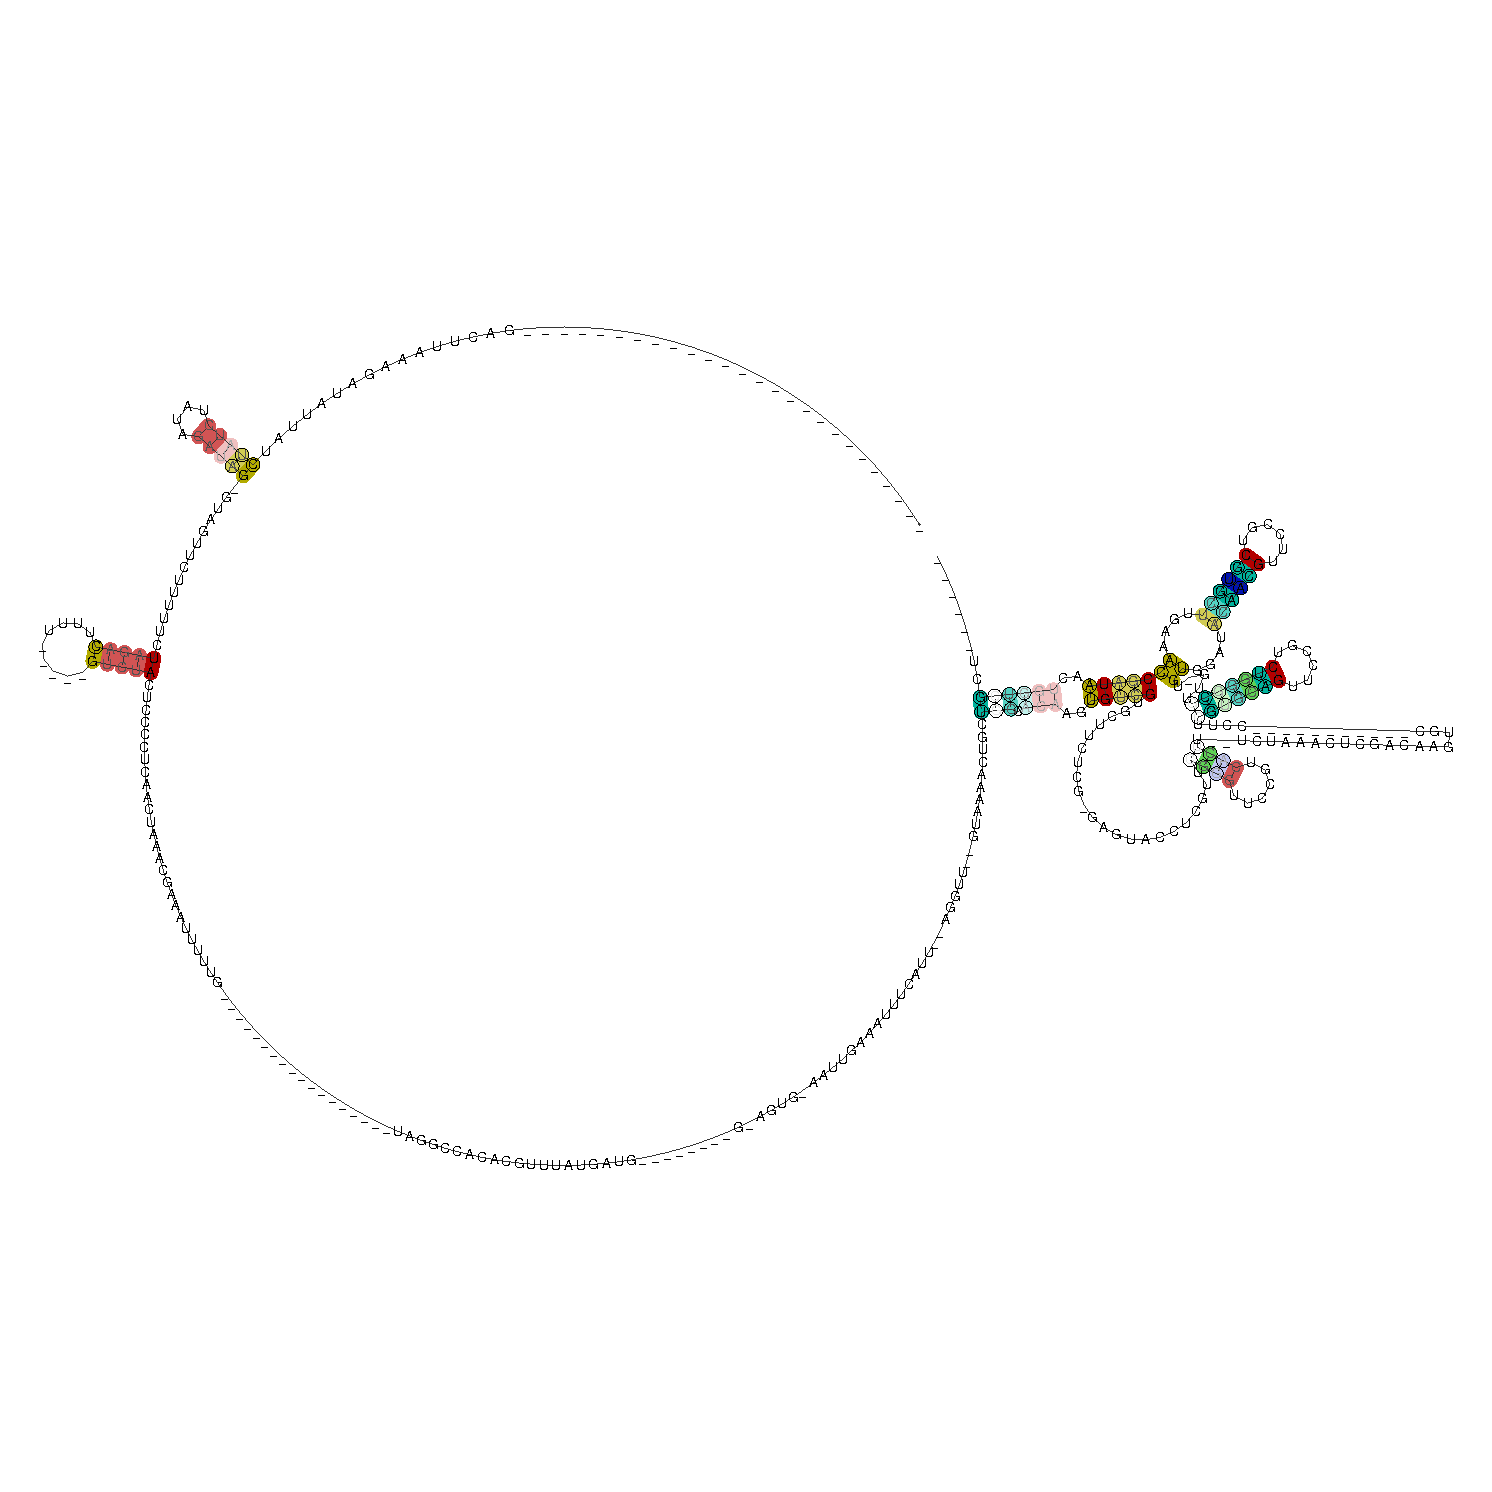
\includegraphics[width=0.75\textwidth]{figures/alirna_mafft.ps}
      \end{minipage} \hfill \begin{minipage}{0.45\textwidth}
      \centering
      \texttt{LocARNA}\\
      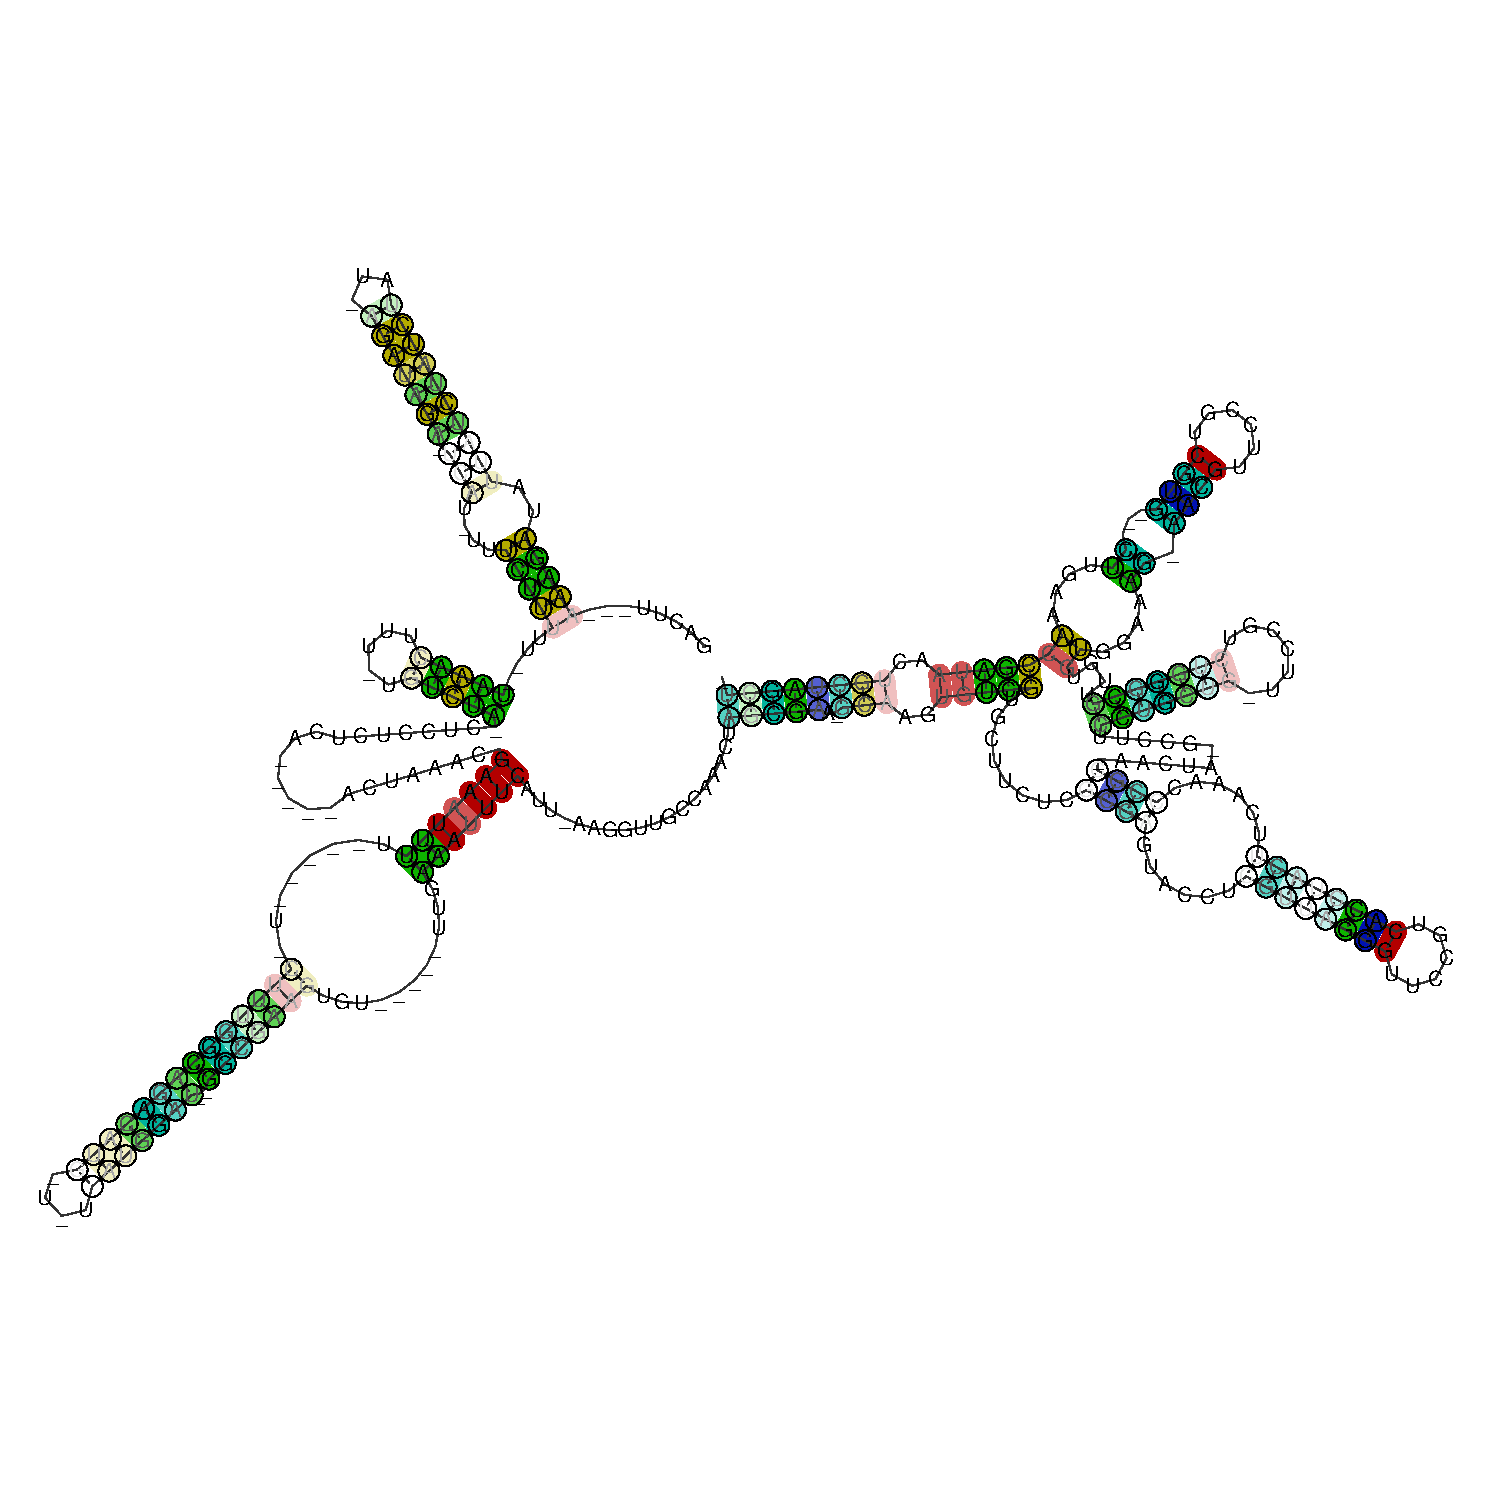
\includegraphics[width=0.75\textwidth]{figures/alirna_locarna.ps}
      \end{minipage}
      }
  
\end{frame}

\begin{frame}[c]\frametitle{VARNA: for nice figures!}
  \begin{figure}[htbp]
      \centering
      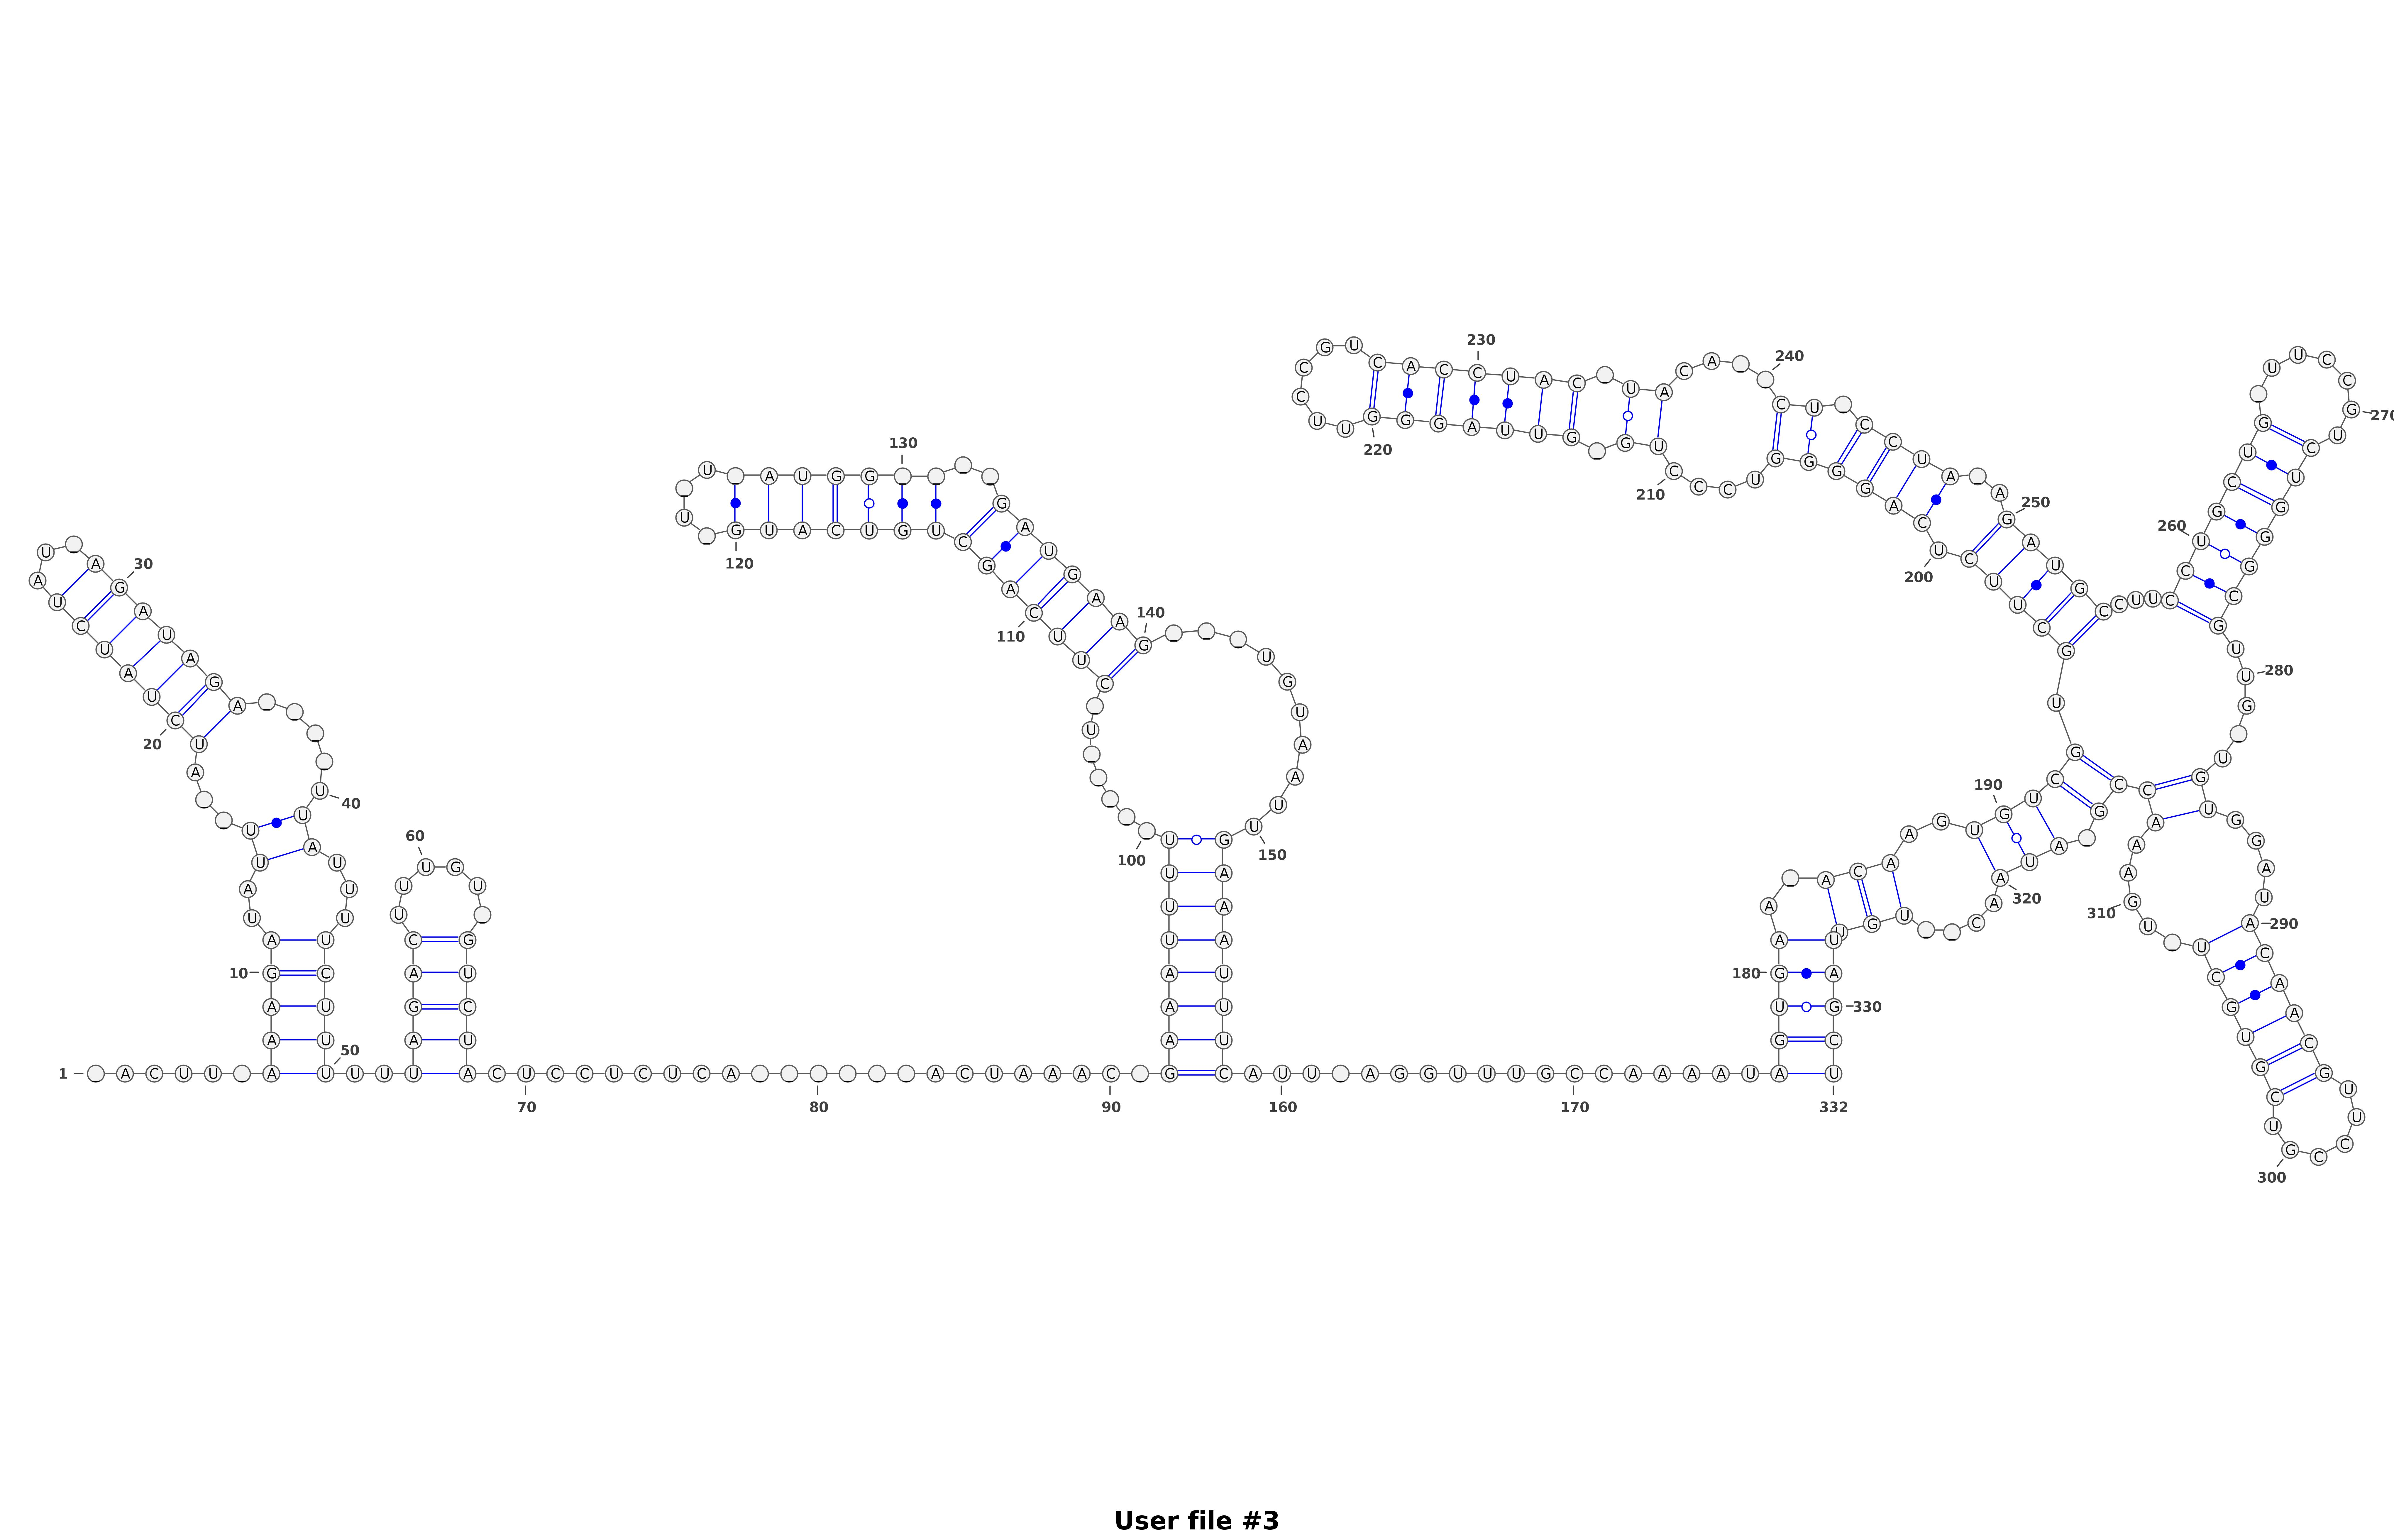
\includegraphics[width=0.95\textwidth]{figures/varna.jpg}        
  \end{figure}
\end{frame}

\begin{frame}[c]\frametitle{RNAalifold Color Code}
  \begin{figure}[htbp]
      \centering
      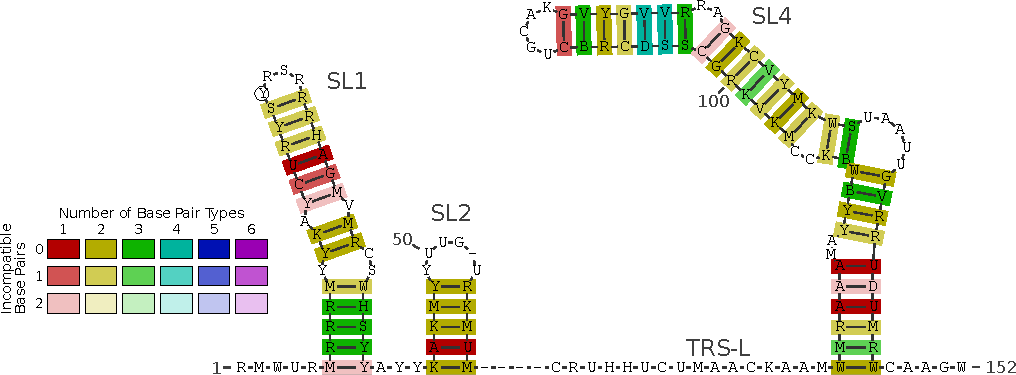
\includegraphics[width=0.95\textwidth]{color_code.pdf}
  \end{figure}
\end{frame}



% Backup Slides. Using this macro, you'd get a slide number for each
% backup slide without increasing the maximum slide numbers of the original presentation.
% However, for this, the framenumber has to be inserted - which isn't in the template by default
\beginbackup

\begin{frame}[c]\frametitle{Coffee Break}
  \begin{figure}[htbp]
    \centering
    
\includegraphics[width=0.65\textwidth]{coffeebreak.png}
  \end{figure}
\end{frame}

\backupend

\end{document}